\documentclass{article}\usepackage[]{graphicx}\usepackage[]{color}
%% maxwidth is the original width if it is less than linewidth
%% otherwise use linewidth (to make sure the graphics do not exceed the margin)
\makeatletter
\def\maxwidth{ %
  \ifdim\Gin@nat@width>\linewidth
    \linewidth
  \else
    \Gin@nat@width
  \fi
}
\makeatother

\definecolor{fgcolor}{rgb}{0.345, 0.345, 0.345}
\newcommand{\hlnum}[1]{\textcolor[rgb]{0.686,0.059,0.569}{#1}}%
\newcommand{\hlstr}[1]{\textcolor[rgb]{0.192,0.494,0.8}{#1}}%
\newcommand{\hlcom}[1]{\textcolor[rgb]{0.678,0.584,0.686}{\textit{#1}}}%
\newcommand{\hlopt}[1]{\textcolor[rgb]{0,0,0}{#1}}%
\newcommand{\hlstd}[1]{\textcolor[rgb]{0.345,0.345,0.345}{#1}}%
\newcommand{\hlkwa}[1]{\textcolor[rgb]{0.161,0.373,0.58}{\textbf{#1}}}%
\newcommand{\hlkwb}[1]{\textcolor[rgb]{0.69,0.353,0.396}{#1}}%
\newcommand{\hlkwc}[1]{\textcolor[rgb]{0.333,0.667,0.333}{#1}}%
\newcommand{\hlkwd}[1]{\textcolor[rgb]{0.737,0.353,0.396}{\textbf{#1}}}%

\usepackage{framed}
\makeatletter
\newenvironment{kframe}{%
 \def\at@end@of@kframe{}%
 \ifinner\ifhmode%
  \def\at@end@of@kframe{\end{minipage}}%
  \begin{minipage}{\columnwidth}%
 \fi\fi%
 \def\FrameCommand##1{\hskip\@totalleftmargin \hskip-\fboxsep
 \colorbox{shadecolor}{##1}\hskip-\fboxsep
     % There is no \\@totalrightmargin, so:
     \hskip-\linewidth \hskip-\@totalleftmargin \hskip\columnwidth}%
 \MakeFramed {\advance\hsize-\width
   \@totalleftmargin\z@ \linewidth\hsize
   \@setminipage}}%
 {\par\unskip\endMakeFramed%
 \at@end@of@kframe}
\makeatother

\definecolor{shadecolor}{rgb}{.97, .97, .97}
\definecolor{messagecolor}{rgb}{0, 0, 0}
\definecolor{warningcolor}{rgb}{1, 0, 1}
\definecolor{errorcolor}{rgb}{1, 0, 0}
\newenvironment{knitrout}{}{} % an empty environment to be redefined in TeX

\usepackage{alltt}
\usepackage[margin=1in]{geometry}
\usepackage{graphicx, hyperref, float, multicol, pdflscape, enumerate, paralist}
\usepackage{amssymb,amsmath,amsthm} 
\usepackage[backend=bibtex, natbib=true]{biblatex}
\addbibresource{../references/references.bib}

\usepackage{color}
\newcommand{\ak}[1]{{\color{magenta} #1}}
\newcommand{\mj}[1]{{\color{blue} #1}}

\theoremstyle{plain}
\newtheorem{res}{Result}

\setlength{\parindent}{0cm}
\renewcommand{\baselinestretch}{1.25}

\title{Bayesian Estimation of the Spectral Density}
\author{Andee Kaplan \& Maggie Johnson}
\IfFileExists{upquote.sty}{\usepackage{upquote}}{}

\begin{document}

\maketitle



\section{Motivation}

To estimate the spectral density of a stationary time series using Bayesian methods using the asymptotic distributional properties of a periodogram. The motivation behind this work is the following model.
\begin{align*}
I_n(\omega_r) |f(\omega_r) &\stackrel{\cdot}{\sim}\text{ indep } \text{Exp}(2\pi f(\omega_r)) \\
f(\omega_r) & \sim \pi(\theta)\\
f(\omega_r) | I_n(\omega_r) &\propto 2\pi f(\omega_r) e^{-2\pi f(\omega_r) y} \pi(\theta)
\end{align*}
The periodogram values at $\omega_r$ are only asymptotically distributed as independent exponentials, so to construct the Bayesian model it is essential that the asymptotic behavior holds. This research uses simulations to \mj{validate} two results by Lahiri. \cite{lahiri2003necessary} \mj{(add if do Bayes, unlikely)}


\section{Background and Problem Statement}

Two results drive the first part of our work.

\begin{res} \label{res:first}
Let $f(\omega_r) \not= 0, 1 \le r \le k$ where $f$ denotes the spectral density of a stationary time series $\{X_t\}$. Then when $n\rightarrow \infty$ the joint distribution of the periodogram at $\omega_r$, $I_n(\omega_r)$, tends to that of $k$ mutually indepependent random variables distributed as $\text{Exponential}(2\pi f(\omega_r))$ for $0<\omega_r<\pi$ \cite{brockwell2002introduction}.
\end{res}

Result~\ref{res:first} describes the asymptotic distribution of a periodogram at fixed frequencies. In practice, this result has often been used with the Fourier frequencies in place of fixed frequencies \mj{reference this} $\{2\pi j/n : j=1,...,n\}$. However, it has been shown that the asymptotic behavior of the periodogram at the Fourier frequencies does not hold as $n \rightarrow \infty$ \mj{(dig into reference to flesh this out)}. Lahiri \cite{lahiri2003necessary} derived two results that describe behavior required for a set of frequencies to satisfy Result~\ref{res:first}

\begin{res} \label{res:lahiri}
In the absense of data tapering,
\begin{enumerate}[(a)]
\item the periodogram values at asymptotically distant ordinates ($I_n(\omega_r)$) are asymptotically independent.  Asymptotically distant ordinates $\{\omega_{ln}\}, \{\omega_{kn}\}$ satisfy $|n(\omega_{ln} - \omega_{kn})| \rightarrow \infty$ as $n \rightarrow \infty$.

\item the periodogram values at asymptotically close ordinates which are asymptotically distant from the sequence $\{0\}$ are asymptotically independent. Asymptotically close ordinates $\{\omega_{ln}\}, \{\omega_{kn}\}$ satisfy $|n(\omega_{ln} - \omega_{kn})| \rightarrow 2\pi l$ for some nonzero integer $l$ as $n \rightarrow \infty$ \cite{lahiri2003necessary}.
\end{enumerate}
\end{res}

%Result~\ref{res:first} gives us the asymptotic distribution of a periodogram at fixed frequencies, while result~\ref{res:lahiri} details properties of frequencies that define where the independence holds. 

Result~\ref{res:lahiri} suggests that for a subset of sufficiently spaced and and distant from 0 frequencies, the periodogram ordinates at these frequencies should be asymptotically independent. \mj{We explore these two results to determine if}, for large $n$,
\begin{enumerate}
  \item Result~\ref{res:first} will not hold at the Fourier frequencies, and
  \item if (1) is true, a subset of Fourier frequencies that are sufficiently spaced and far from 0 can be constructed such that Result~\ref{res:first} holds.
\end{enumerate}

%at at what point distant from zero and at what spacings close to zero do the approximate independence and exponential distribution fail in the periodogram values. 



\section{Models}

\mj{WHAT ARE WE DOING?!?!}

We used three separate models to explore the asymptotic behavior of the periodogram. The included models are \begin{inparaenum}[\itshape a\upshape)]
\item IID Gaussian(0, 1);
\item AR(1) with $\phi = 0.5$; and
\item AR(4) with $\boldsymbol{\phi} = [0.08, 0.33, 0.1, 0.45$].
\end{inparaenum}

\subsubsection*{IID Gaussian}
The following result about the IID Gaussian model gives us knowledge of the exact, rather than asymptotic, behavior of the periodogram at any frequency.

\begin{res}
For $\{X_t\} \stackrel{\text{IID}}{\sim} \text{N}(0,\sigma^2)$, the periodogram values $\left\{ I_n(\omega_j): \omega_j \in \mathcal{F}_n, \omega_j \not\in \{0,\pi\} \right\}$ are IID Exponential($\sigma^2$) random variables \cite{brockwell2002introduction}.
\end{res}

We use this model as a sanity check on our testing procedure. Should our procedure show failure with the IID Gaussian model, then this is an indication of an issue with the procedure, rather than the frequency spacings.

\subsubsection*{ARMA(p,q)}
We used exclusively ARMA models as our experimental models because the spectral density of an ARMA model has a known and closed form. An ARMA model is a process $\{X_t\}$ with the form $\phi(B)X_t = \theta(B)Z_t$ where $B$ is the backshift operator and $\{Z_t\}$ is WN(0,$\sigma^2$). Models of this form have spectral density

\begin{align*}
f_X(\omega) = \frac{\sigma^2}{2\pi} \frac{|\theta(e^{-i \omega})|^2}{|\phi(e^{-i \omega})|^2}, \omega \in [-\pi, \pi] \text{\cite{brockwell2002introduction}}.
\end{align*}

Without the exact knowledge of the spectral density function, we would not be able to test the distributions of the periodogram at each fequencies. \mj{mention moving window?}


\section{Procedures}

\mj{Explain two tests for independence and exponentials, pairwise tests even though not necessarily joint independence}
We implement the following testing procedure and repeat $s$ simulations of the tests to determine if we see similar rates of failures as the Type-I errors of our tests ($\alpha$).

\begin{enumerate}
\item Simulate $M$ draws from $X_1,\dots, X_n$ where $\{X_t\}$ is a stationary time series from one of three models.
\item \label{perio}Obtain $M$ periodograms using the fourier frequencies from $(0, \pi)$, $\omega_j = \frac{2\pi j}{n}: j = 1, \dots, \lfloor n/2 \rfloor$.
\item Obtain $\lfloor\frac{n-1}{2}\rfloor$ values of the spectral density at each fourier frequency $f(\omega_j)$. These will be known by design.
\item Simulate $M$ draws from the $\lfloor\frac{n-1}{2}\rfloor$ different distributions $\text{Exp}(2\pi f(\omega_r))$
\item \label{test:exp}Test the distribution of the $M$ values of periodograms at each fourier frequency separately. Store the number of failed tests at each frequency.
\item \label{test:indep}Test the pairwise independence of each neighboring $M$ values of periodograms at each fourier frequency. Store the number of failed tests at each frequency.
\item Inspect the results from steps~\ref{test:exp} and \ref{test:indep} to determine if different spacings of frequencies are needed. If so, use sparcer frequencies and repeat from step~\ref{perio} at the chosen frequencies rather than fourier frequencies.
\end{enumerate}


\subsection{Tests}



\paragraph{Spearman's Rank Correlation}



\paragraph{Kolmogorov-Smirnov Test of Distribution}






\section{Results}




\subsection*{IID Gaussian}
\begin{knitrout}
\definecolor{shadecolor}{rgb}{0.969, 0.969, 0.969}\color{fgcolor}\begin{figure}[H]

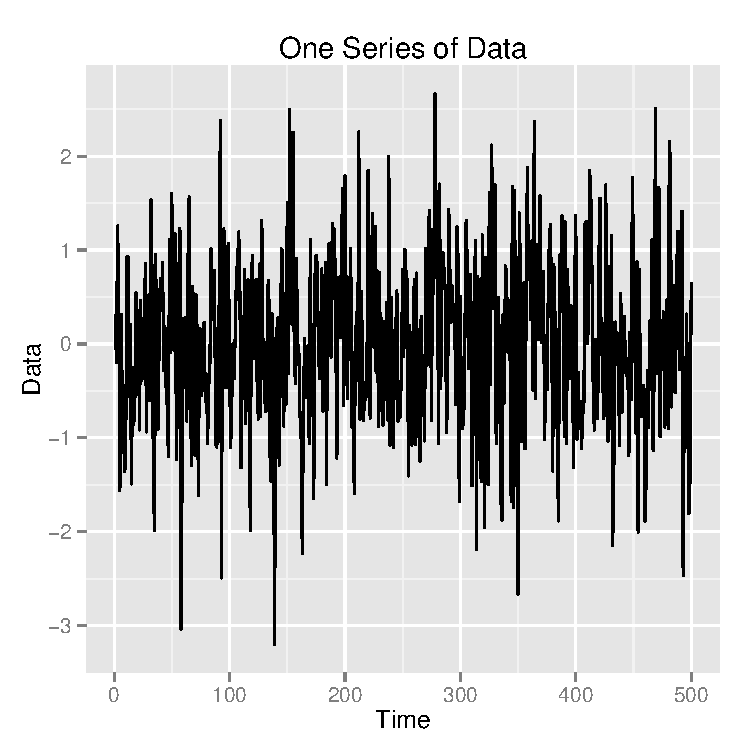
\includegraphics[width=.33\textwidth]{figure/inital-iid1} 
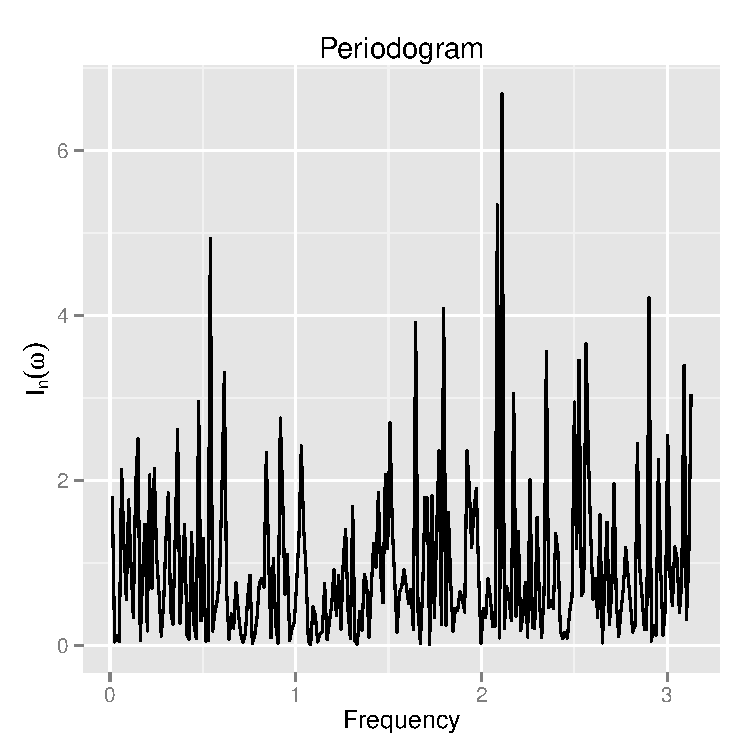
\includegraphics[width=.33\textwidth]{figure/inital-iid2} 
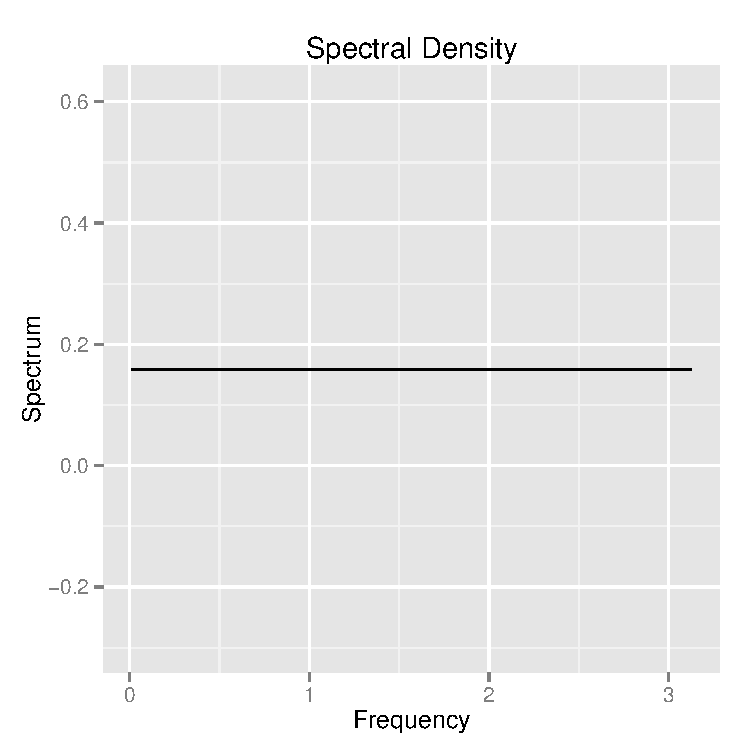
\includegraphics[width=.33\textwidth]{figure/inital-iid3} \caption[One draw, periodogram, and spectral density of a Gaussian IID Model]{One draw, periodogram, and spectral density of a Gaussian IID Model.\label{fig:inital-iid}}
\end{figure}


\end{knitrout}


\begin{knitrout}
\definecolor{shadecolor}{rgb}{0.969, 0.969, 0.969}\color{fgcolor}\begin{figure}[H]

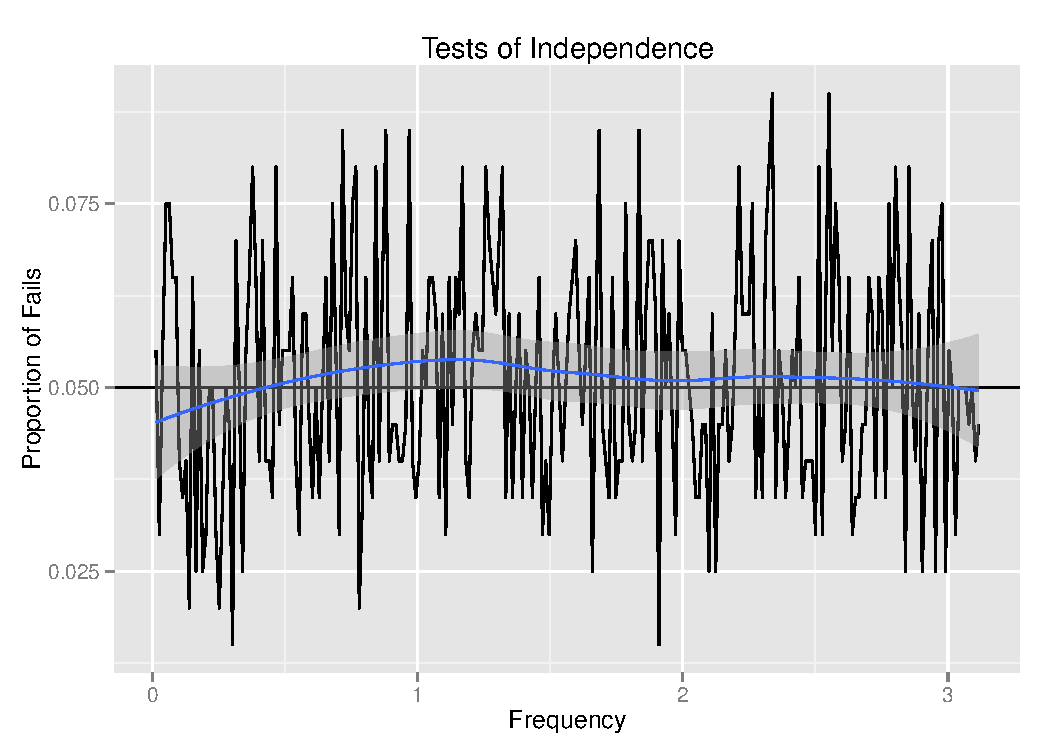
\includegraphics[width=.49\textwidth]{figure/tests-iid1} 
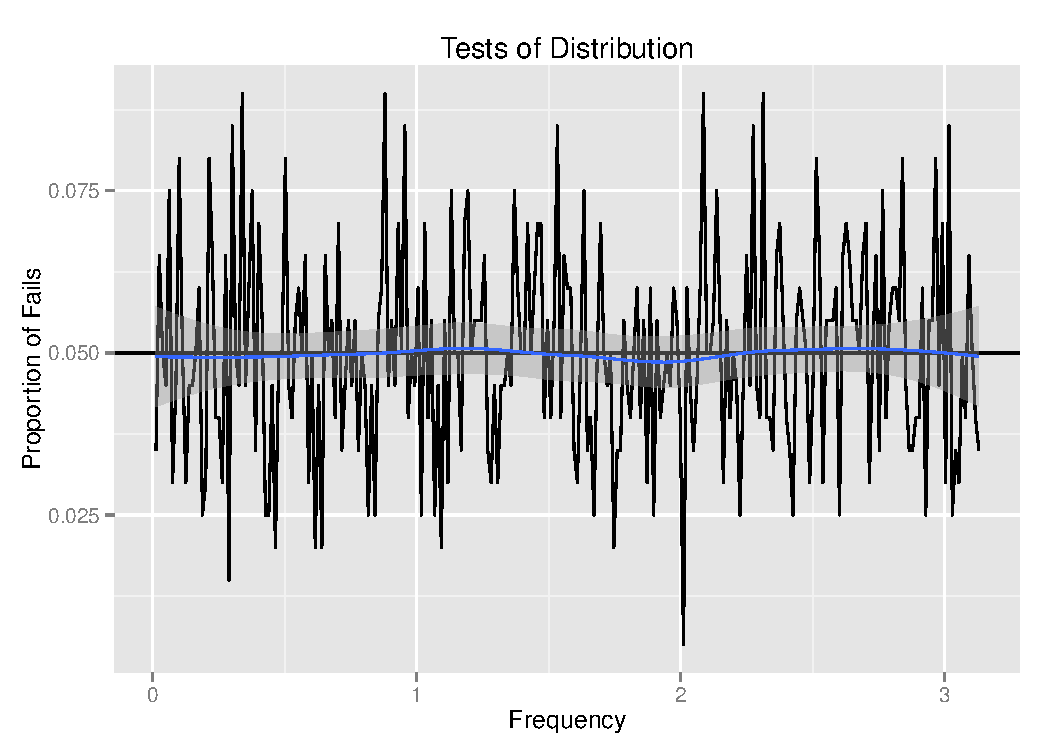
\includegraphics[width=.49\textwidth]{figure/tests-iid2} \caption[Tests of independence and distribution for a Gaussian IID Model]{Tests of independence and distribution for a Gaussian IID Model.\label{fig:tests-iid}}
\end{figure}


\end{knitrout}


\subsection*{AR(1)}
\begin{knitrout}
\definecolor{shadecolor}{rgb}{0.969, 0.969, 0.969}\color{fgcolor}\begin{figure}[H]

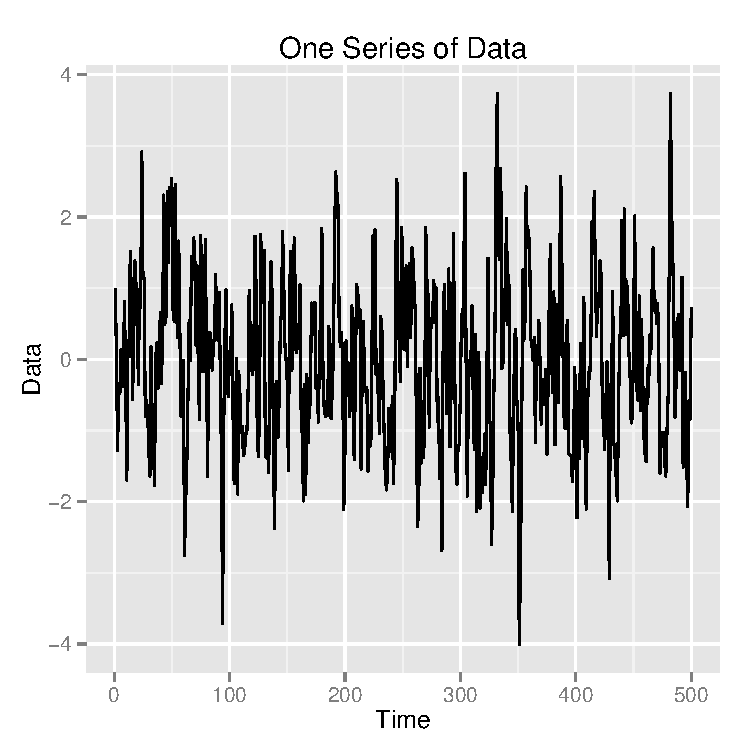
\includegraphics[width=.33\textwidth]{figure/inital-ar11} 
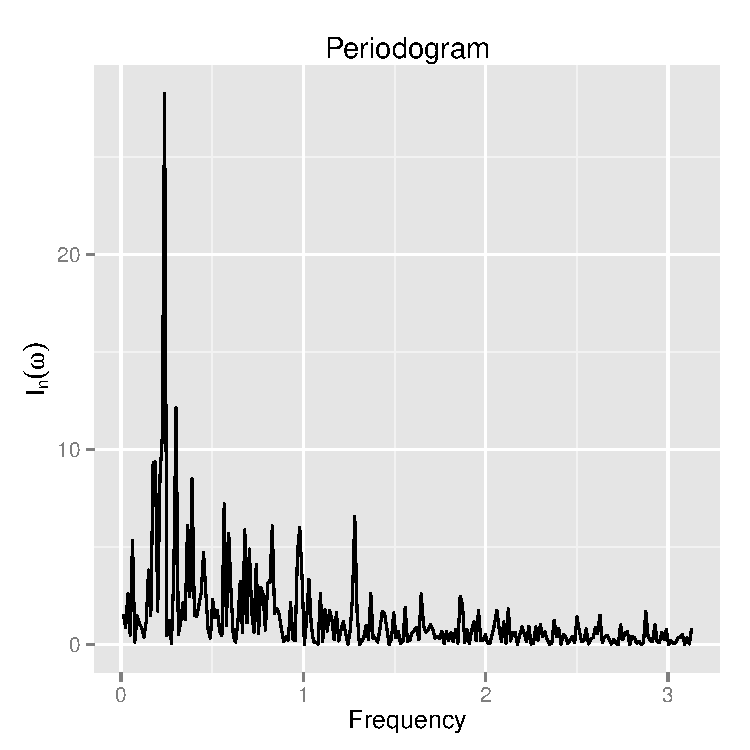
\includegraphics[width=.33\textwidth]{figure/inital-ar12} 
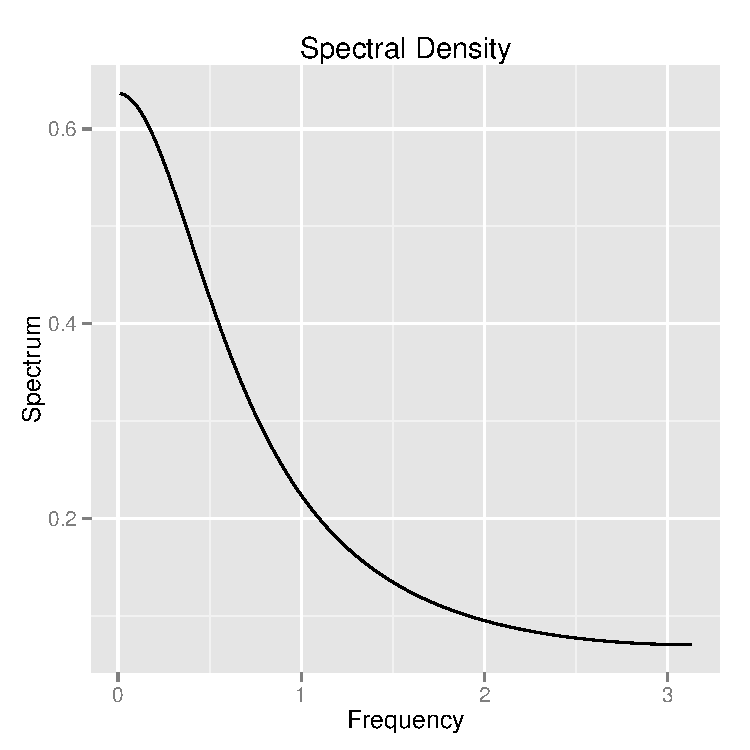
\includegraphics[width=.33\textwidth]{figure/inital-ar13} \caption[One draw, periodogram, and spectral density of an AR(1) model]{One draw, periodogram, and spectral density of an AR(1) model.\label{fig:inital-ar1}}
\end{figure}


\end{knitrout}


\begin{knitrout}
\definecolor{shadecolor}{rgb}{0.969, 0.969, 0.969}\color{fgcolor}\begin{figure}[H]

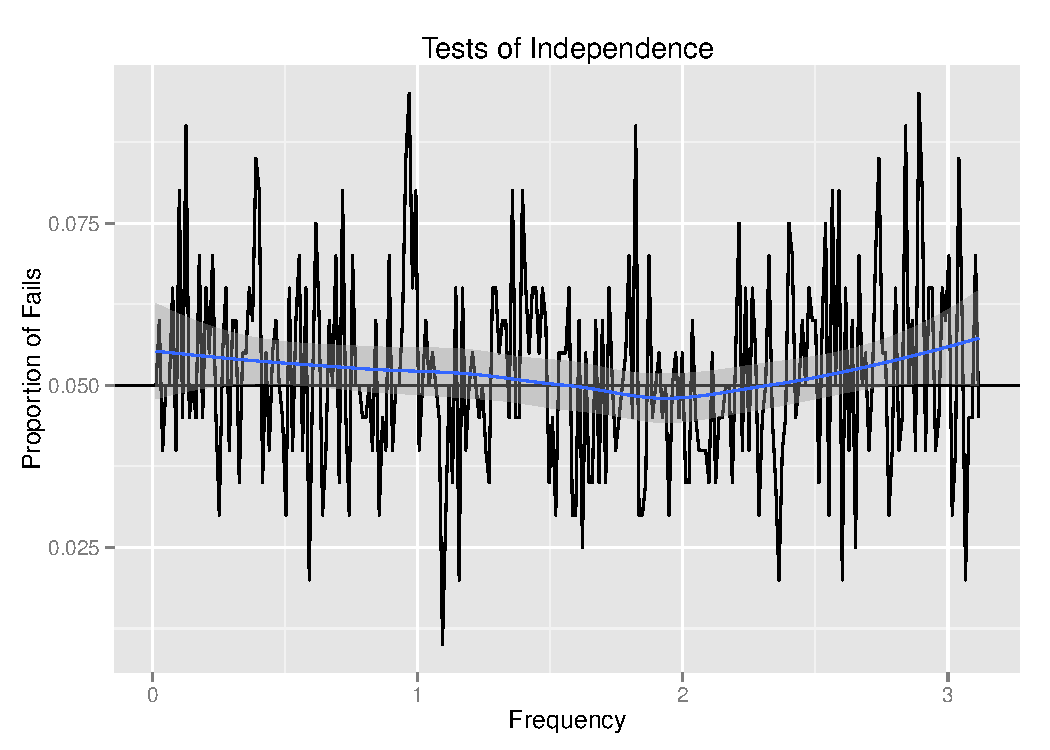
\includegraphics[width=.49\textwidth]{figure/tests-ar11} 
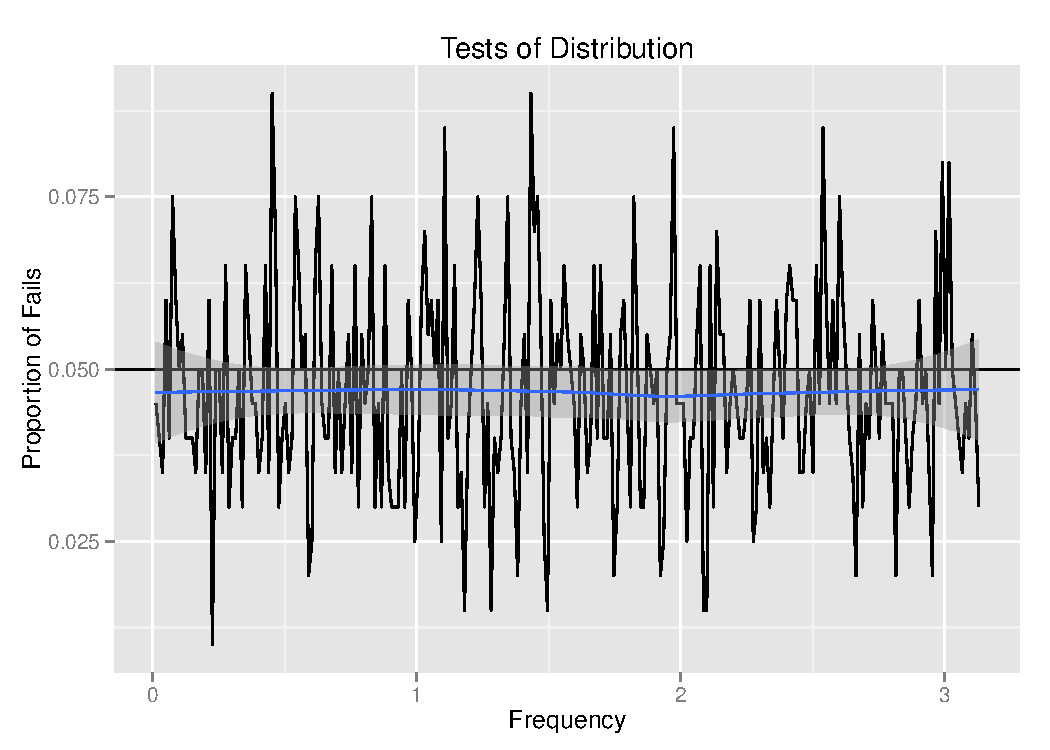
\includegraphics[width=.49\textwidth]{figure/tests-ar12} \caption[Tests of independence and distribution for an AR(1) model]{Tests of independence and distribution for an AR(1) model.\label{fig:tests-ar1}}
\end{figure}


\end{knitrout}


\subsection*{AR(4)}
\begin{knitrout}
\definecolor{shadecolor}{rgb}{0.969, 0.969, 0.969}\color{fgcolor}\begin{figure}[H]

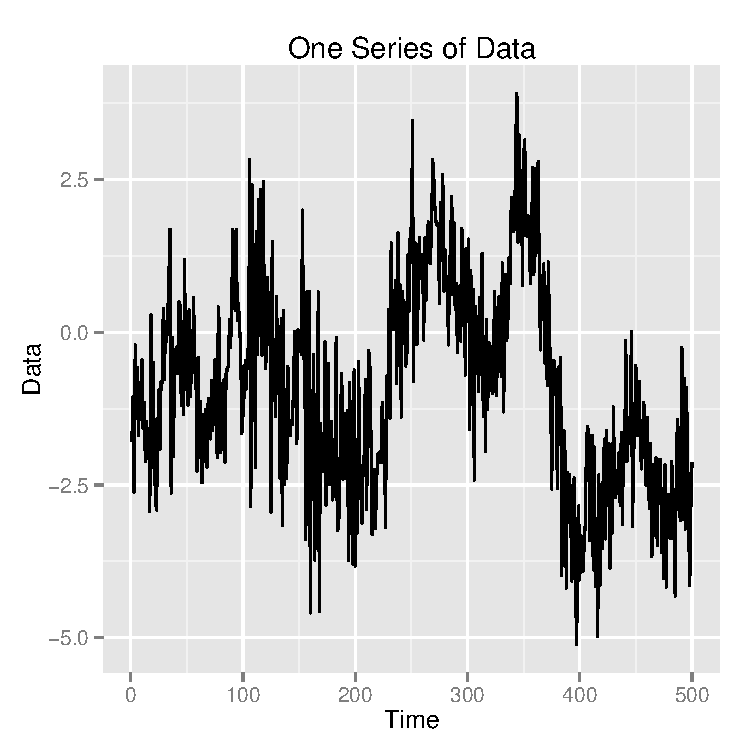
\includegraphics[width=.33\textwidth]{figure/inital-ar41} 
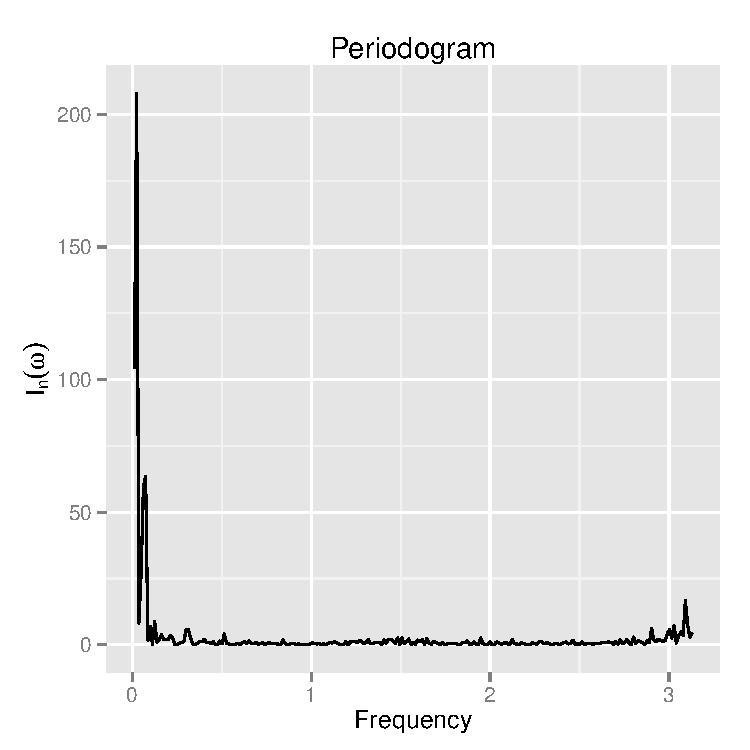
\includegraphics[width=.33\textwidth]{figure/inital-ar42} 
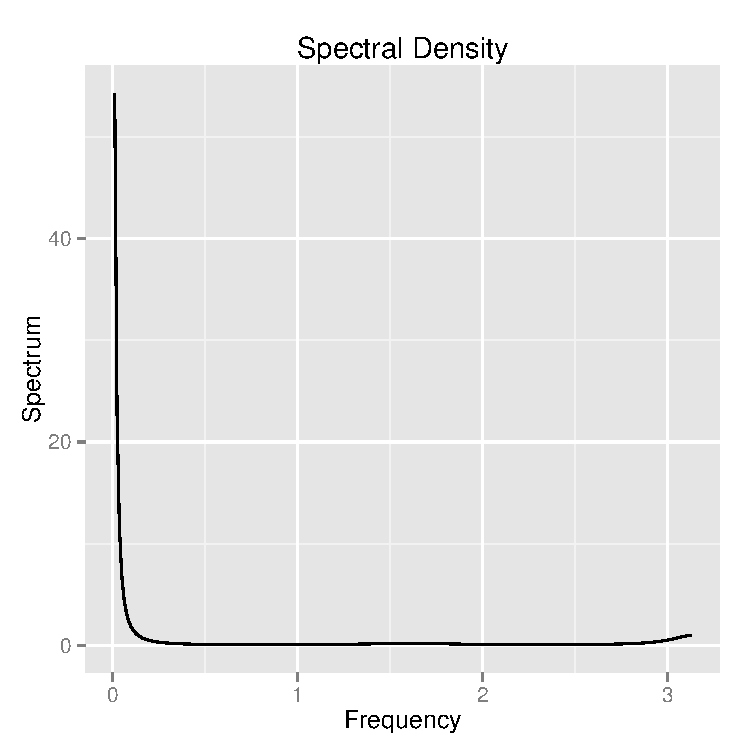
\includegraphics[width=.33\textwidth]{figure/inital-ar43} \caption[One draw, periodogram, and spectral density of an AR(4) model]{One draw, periodogram, and spectral density of an AR(4) model.\label{fig:inital-ar4}}
\end{figure}


\end{knitrout}


\begin{knitrout}
\definecolor{shadecolor}{rgb}{0.969, 0.969, 0.969}\color{fgcolor}\begin{figure}[H]

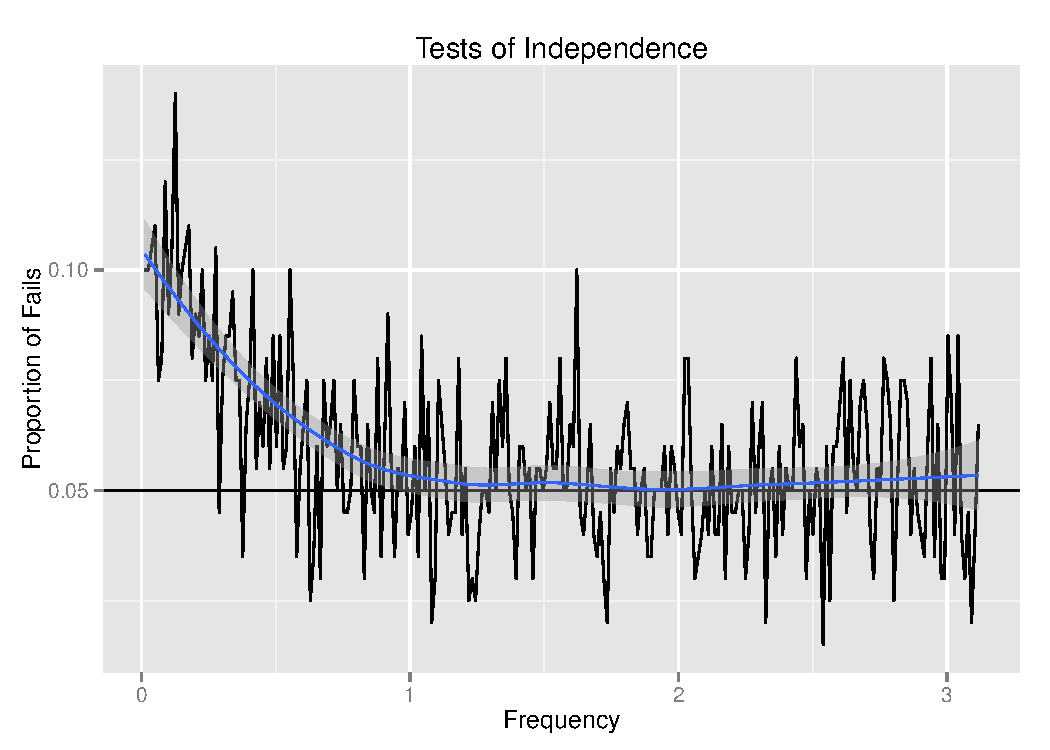
\includegraphics[width=.49\textwidth]{figure/tests-ar41} 
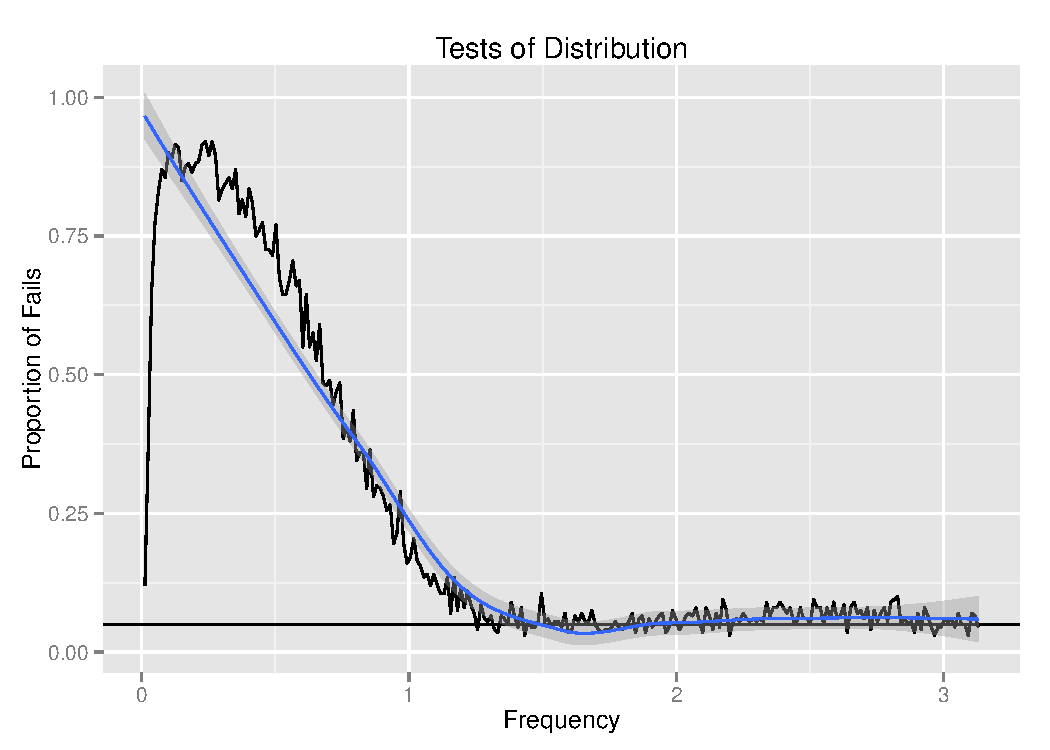
\includegraphics[width=.49\textwidth]{figure/tests-ar42} \caption[Tests of independence and distribution for an AR(4) model]{Tests of independence and distribution for an AR(4) model.\label{fig:tests-ar4}}
\end{figure}


\end{knitrout}


\subsection*{MA(1)}
\begin{knitrout}
\definecolor{shadecolor}{rgb}{0.969, 0.969, 0.969}\color{fgcolor}\begin{figure}[H]

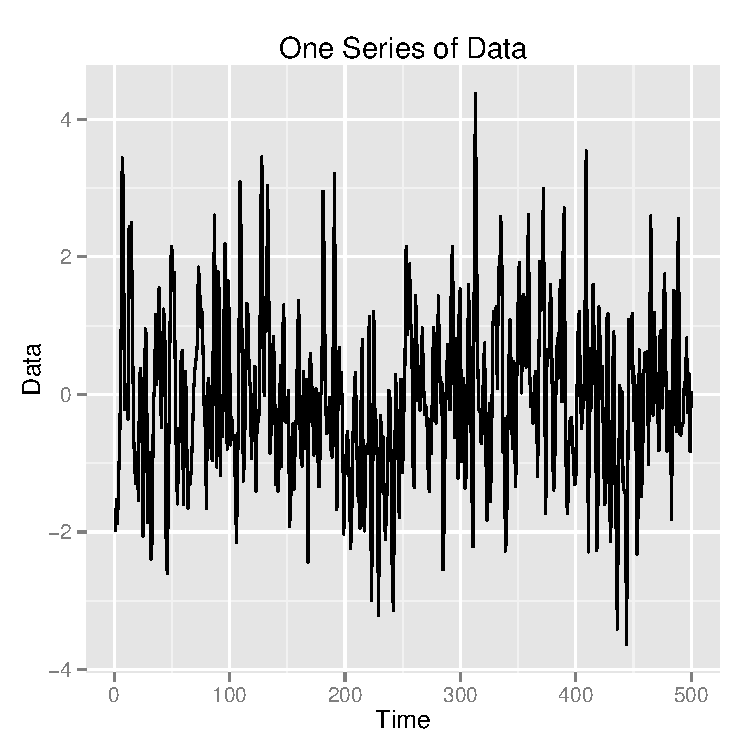
\includegraphics[width=.33\textwidth]{figure/inital-ma11} 
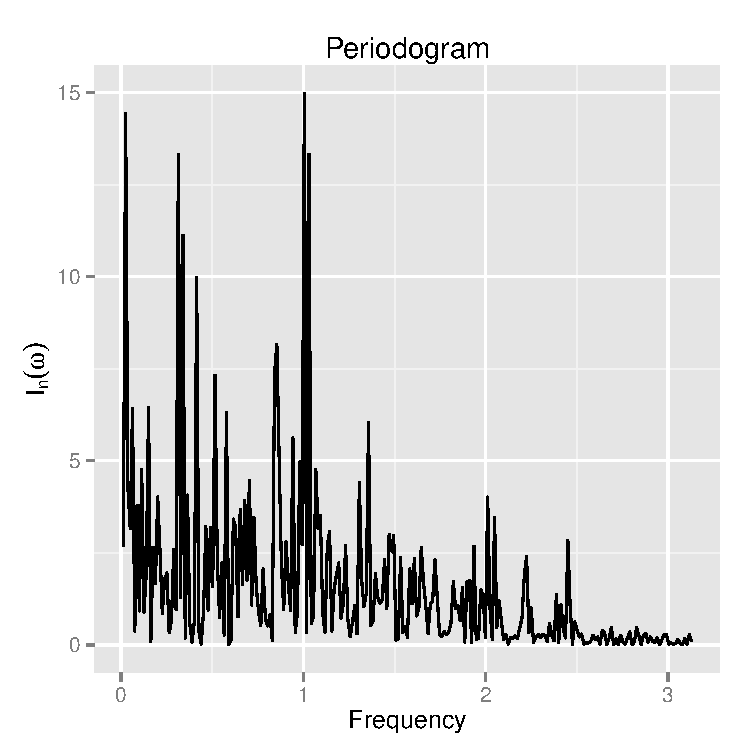
\includegraphics[width=.33\textwidth]{figure/inital-ma12} 
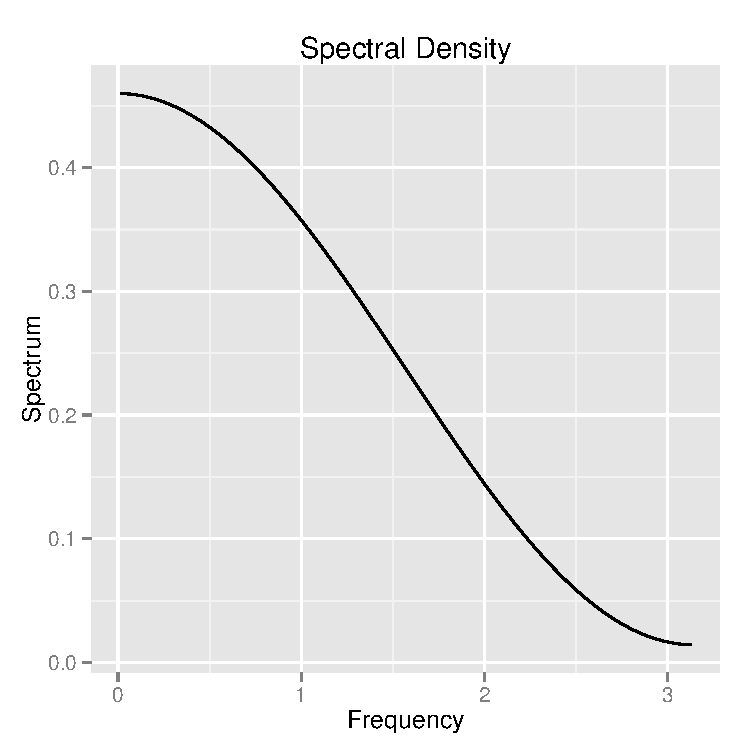
\includegraphics[width=.33\textwidth]{figure/inital-ma13} \caption[One draw, periodogram, and spectral density of an MA(1) model]{One draw, periodogram, and spectral density of an MA(1) model.\label{fig:inital-ma1}}
\end{figure}


\end{knitrout}


\begin{knitrout}
\definecolor{shadecolor}{rgb}{0.969, 0.969, 0.969}\color{fgcolor}\begin{figure}[H]

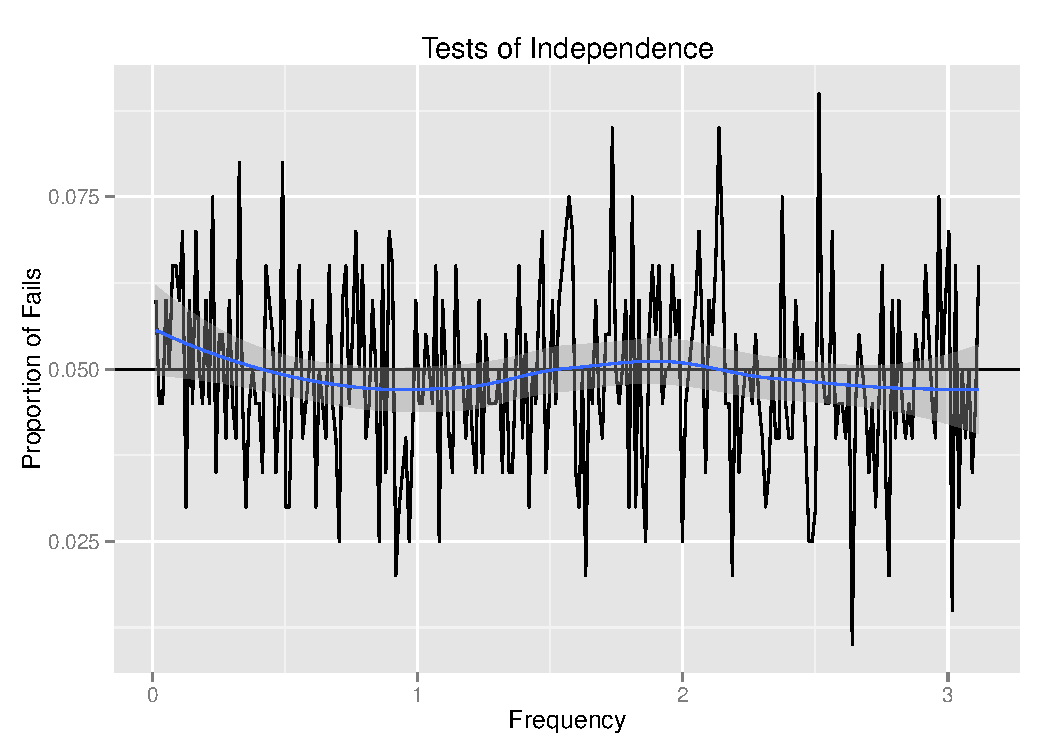
\includegraphics[width=.49\textwidth]{figure/tests-ma11} 
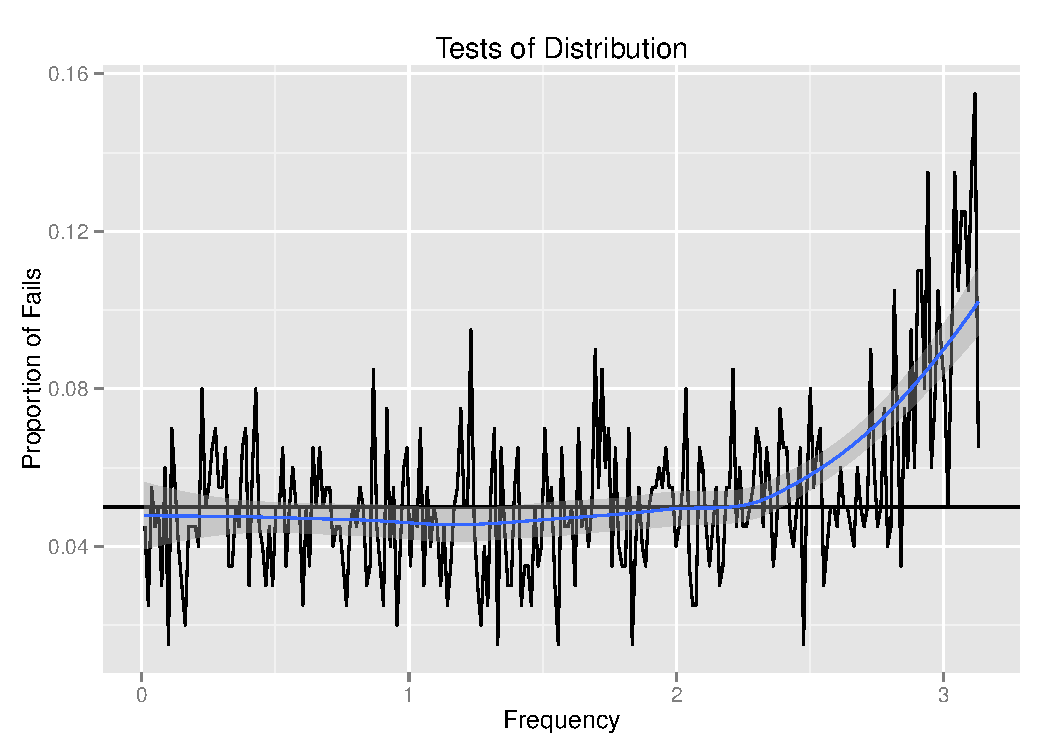
\includegraphics[width=.49\textwidth]{figure/tests-ma12} \caption[Tests of independence and distribution for an MA(1) model]{Tests of independence and distribution for an MA(1) model.\label{fig:tests-ma1}}
\end{figure}


\end{knitrout}


\subsection*{MA(2)}
\begin{knitrout}
\definecolor{shadecolor}{rgb}{0.969, 0.969, 0.969}\color{fgcolor}\begin{figure}[H]

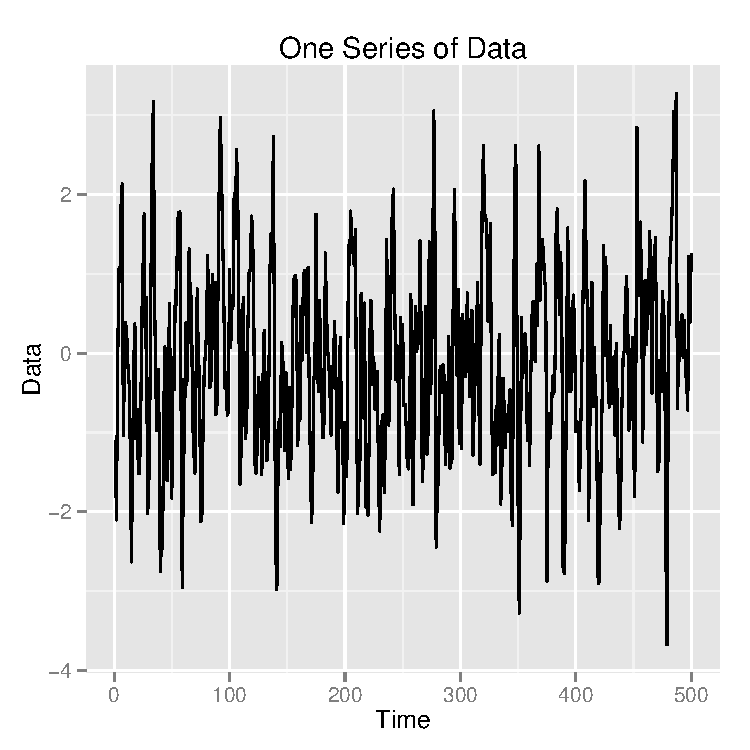
\includegraphics[width=.33\textwidth]{figure/inital-ma21} 
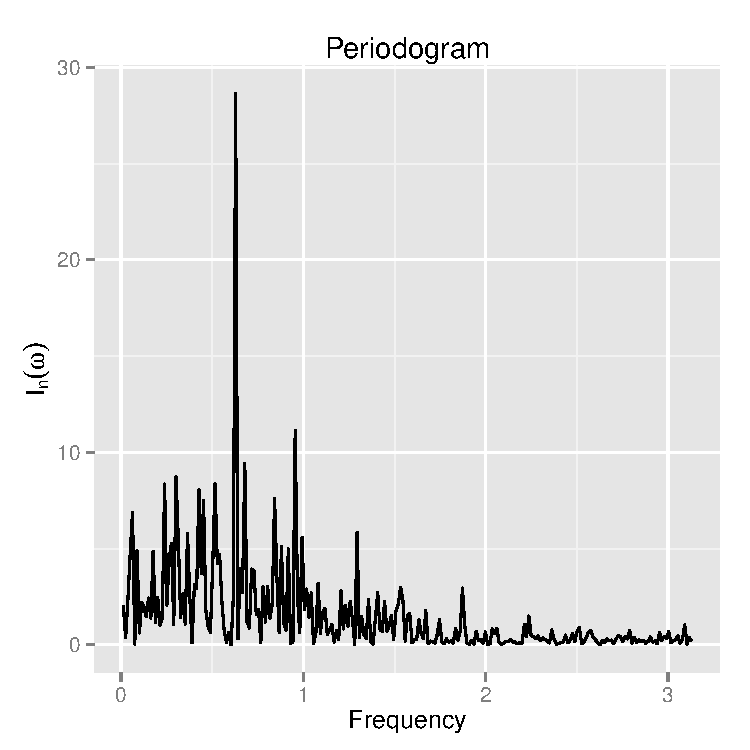
\includegraphics[width=.33\textwidth]{figure/inital-ma22} 
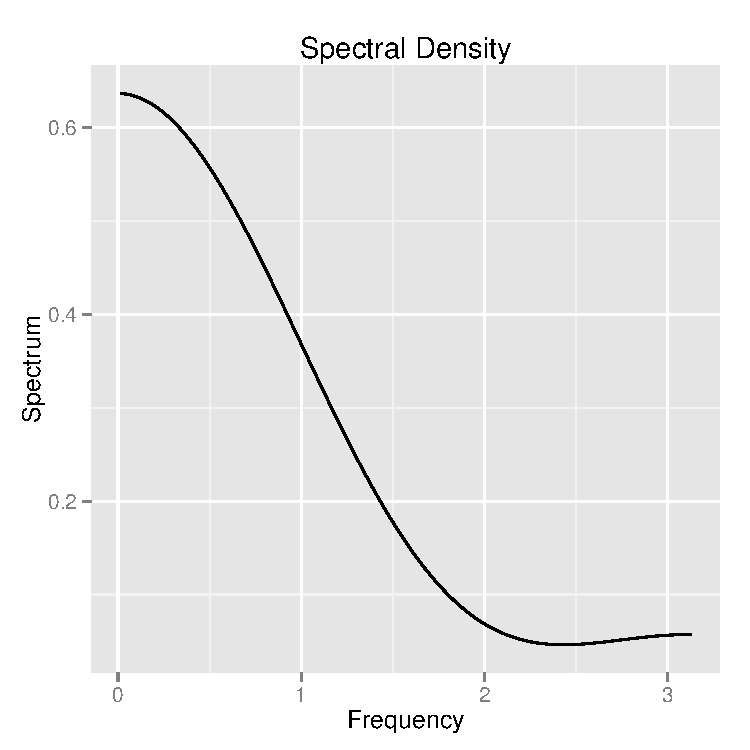
\includegraphics[width=.33\textwidth]{figure/inital-ma23} \caption[One draw, periodogram, and spectral density of an MA(2) model]{One draw, periodogram, and spectral density of an MA(2) model.\label{fig:inital-ma2}}
\end{figure}


\end{knitrout}


\begin{knitrout}
\definecolor{shadecolor}{rgb}{0.969, 0.969, 0.969}\color{fgcolor}\begin{figure}[H]

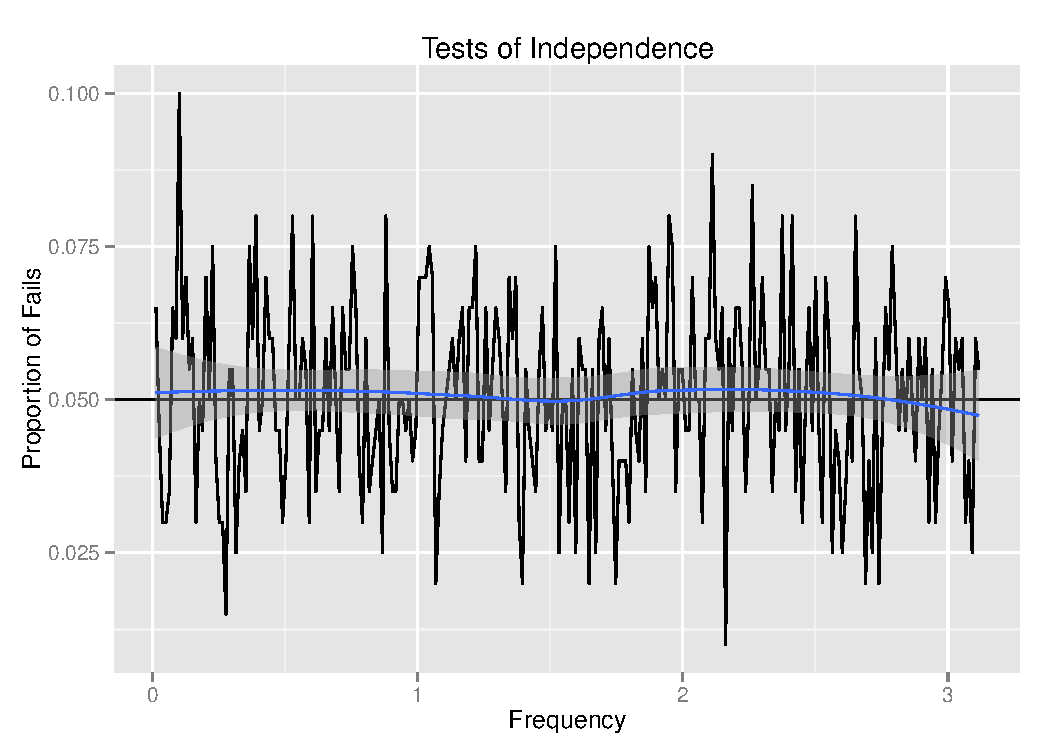
\includegraphics[width=.49\textwidth]{figure/tests-ma21} 
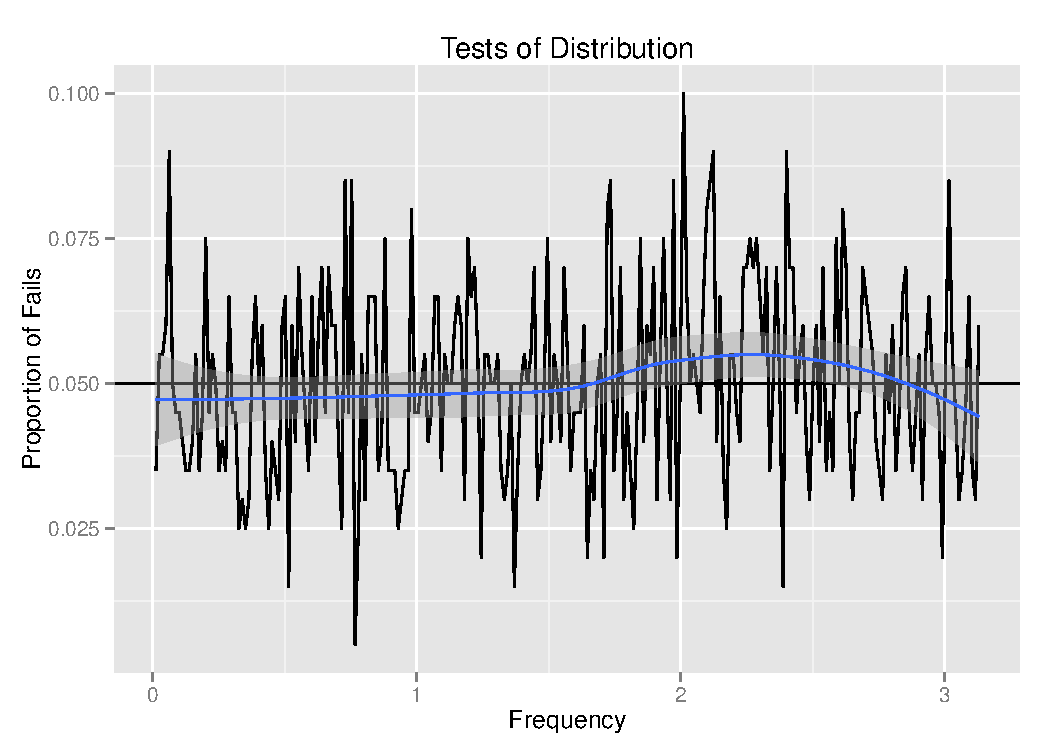
\includegraphics[width=.49\textwidth]{figure/tests-ma22} \caption[Tests of independence and distribution for an MA(2) model]{Tests of independence and distribution for an MA(2) model.\label{fig:tests-ma2}}
\end{figure}


\end{knitrout}


\subsection*{ARMA(4,1)}
\begin{knitrout}
\definecolor{shadecolor}{rgb}{0.969, 0.969, 0.969}\color{fgcolor}\begin{figure}[H]

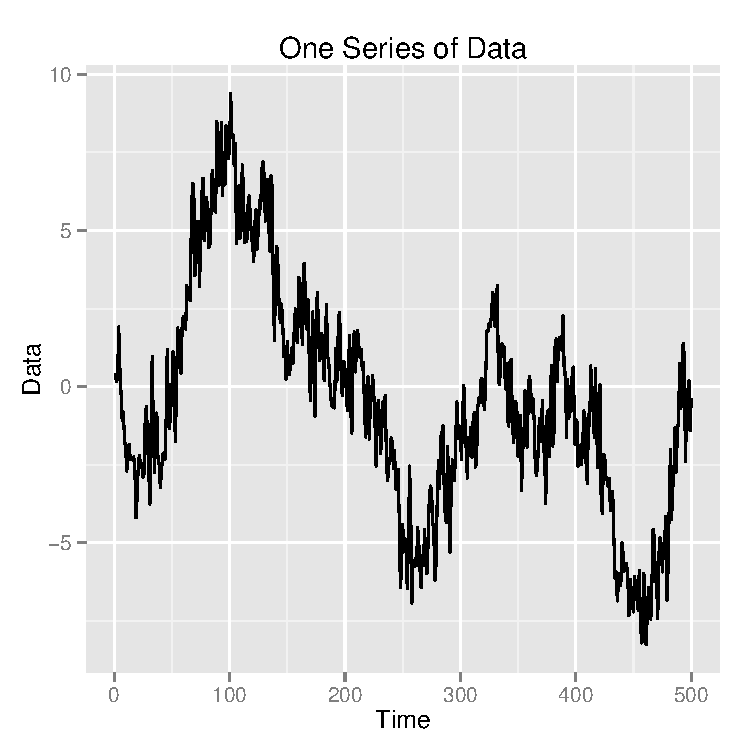
\includegraphics[width=.33\textwidth]{figure/inital-arma411} 
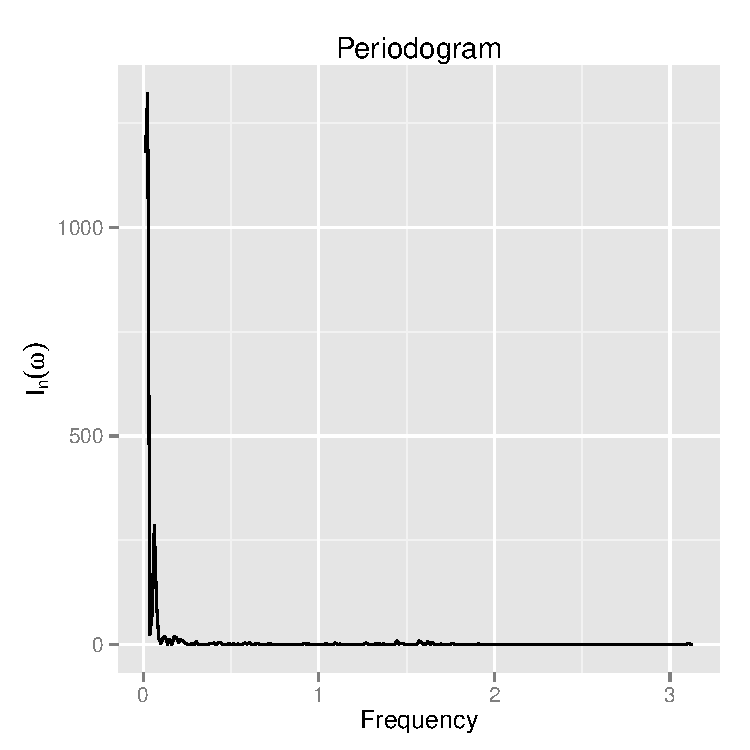
\includegraphics[width=.33\textwidth]{figure/inital-arma412} 
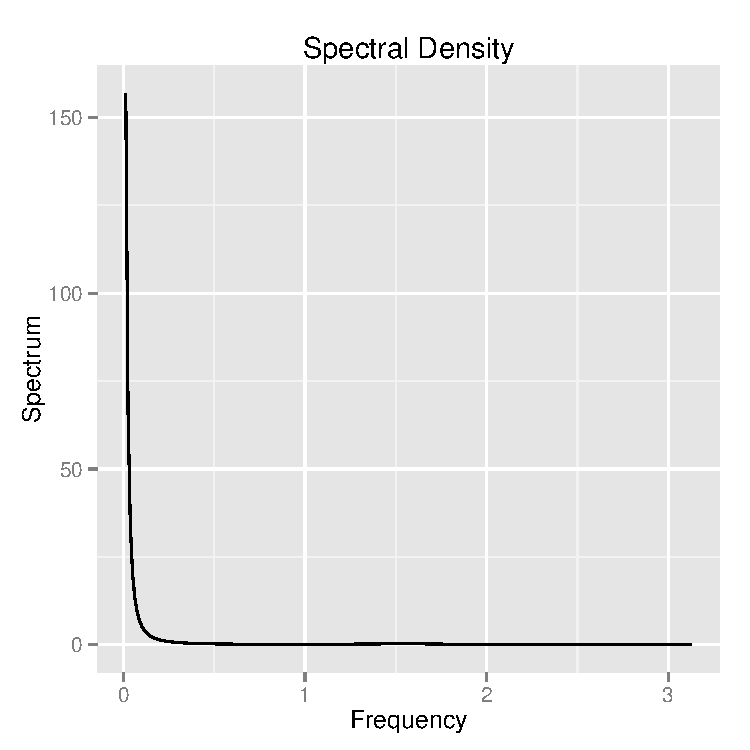
\includegraphics[width=.33\textwidth]{figure/inital-arma413} \caption[One draw, periodogram, and spectral density of an ARMA(4,1) model]{One draw, periodogram, and spectral density of an ARMA(4,1) model.\label{fig:inital-arma41}}
\end{figure}


\end{knitrout}


\begin{knitrout}
\definecolor{shadecolor}{rgb}{0.969, 0.969, 0.969}\color{fgcolor}\begin{figure}[H]

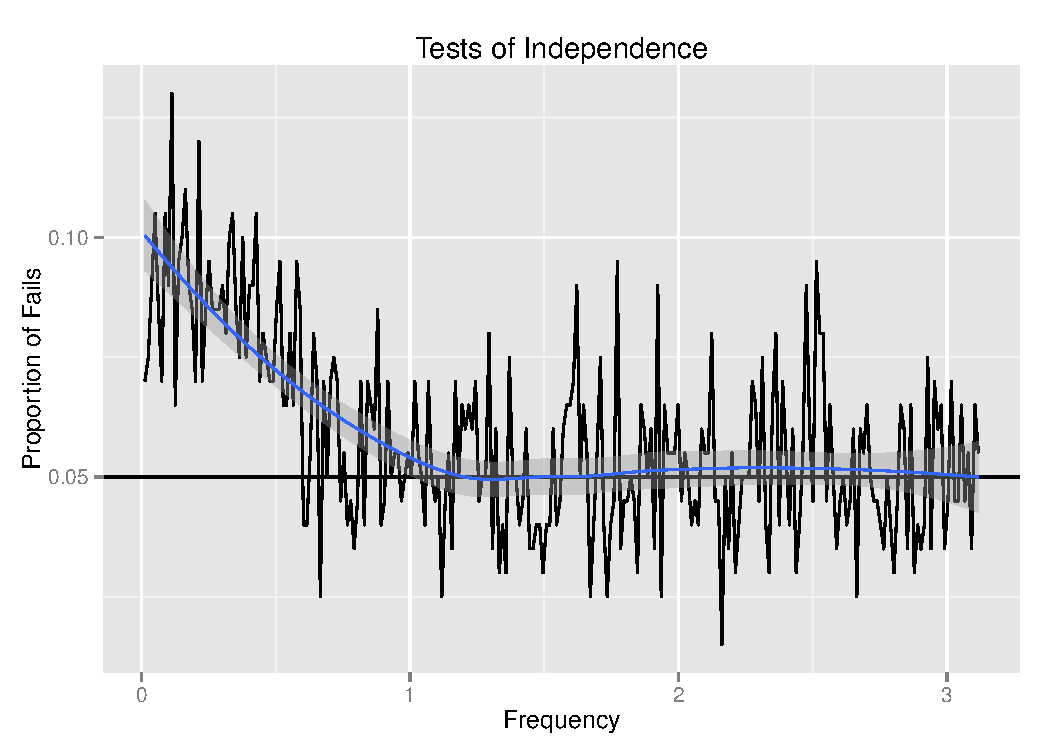
\includegraphics[width=.49\textwidth]{figure/tests-arma411} 
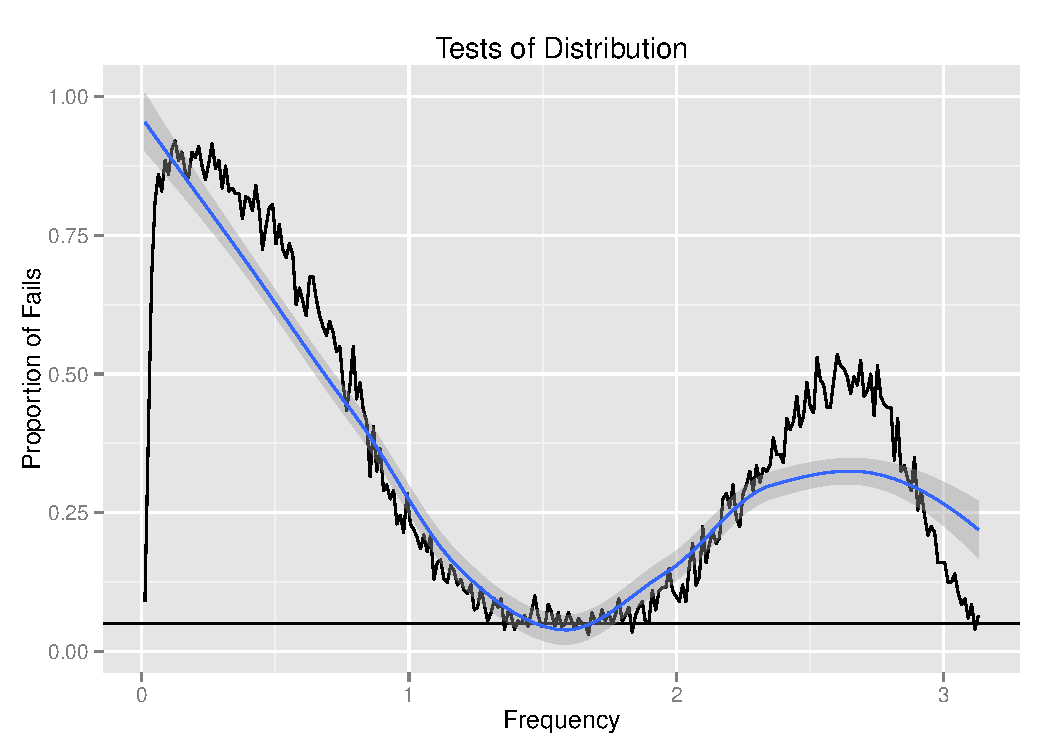
\includegraphics[width=.49\textwidth]{figure/tests-arma412} \caption[Tests of independence and distribution for an ARMA(4,1) model]{Tests of independence and distribution for an ARMA(4,1) model.\label{fig:tests-arma41}}
\end{figure}


\end{knitrout}


\subsection*{ARMA(4,2)}
\begin{knitrout}
\definecolor{shadecolor}{rgb}{0.969, 0.969, 0.969}\color{fgcolor}\begin{figure}[H]

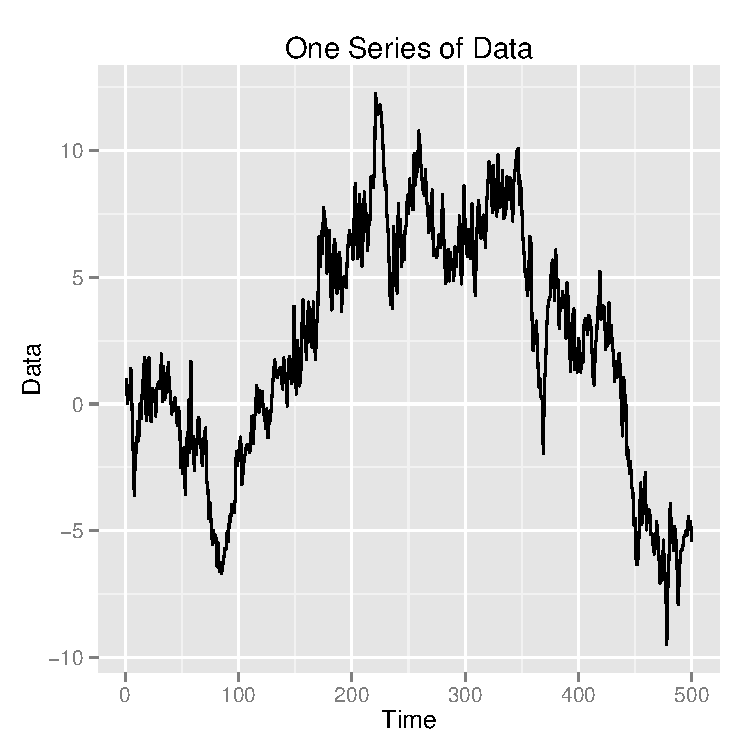
\includegraphics[width=.33\textwidth]{figure/inital-arma421} 
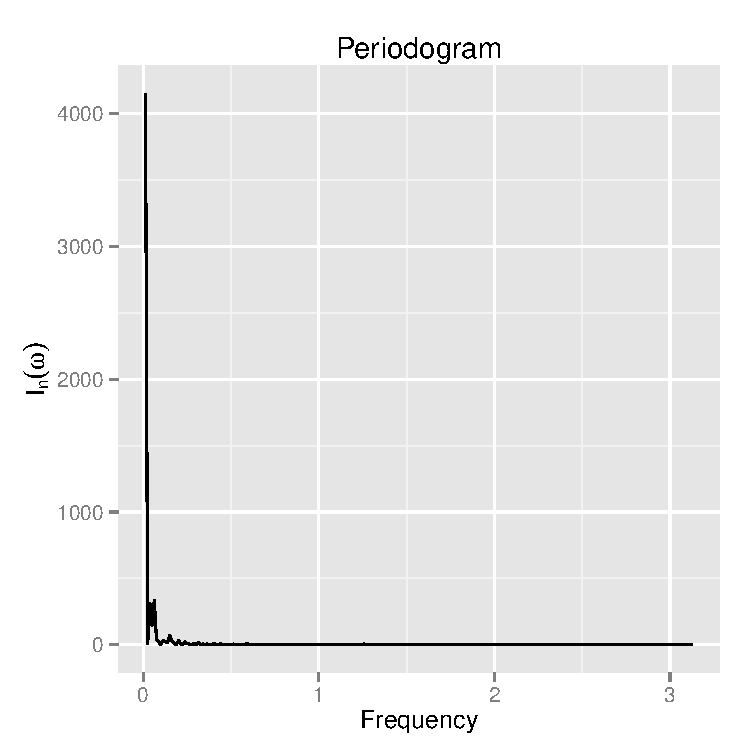
\includegraphics[width=.33\textwidth]{figure/inital-arma422} 
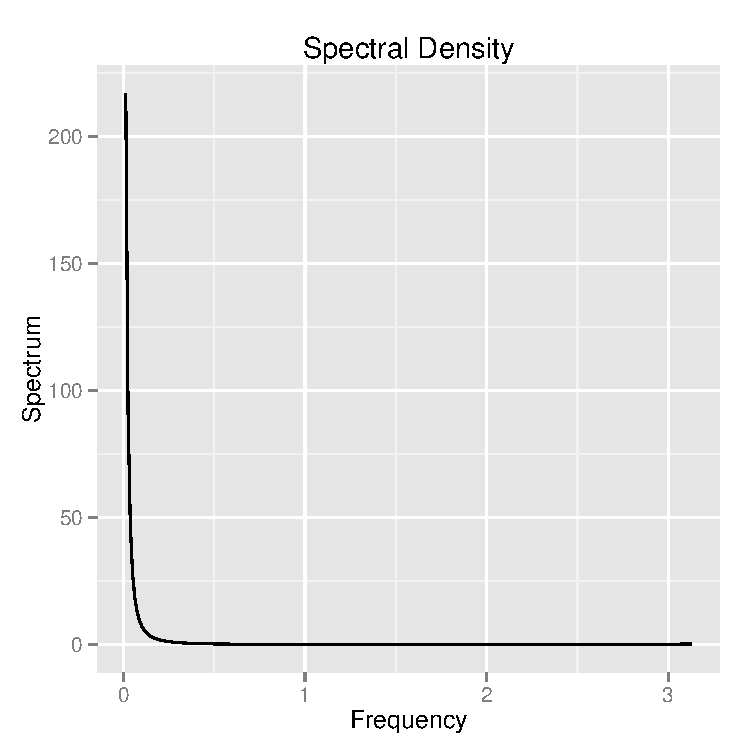
\includegraphics[width=.33\textwidth]{figure/inital-arma423} \caption[One draw, periodogram, and spectral density of an ARMA(4,2) model]{One draw, periodogram, and spectral density of an ARMA(4,2) model.\label{fig:inital-arma42}}
\end{figure}


\end{knitrout}


\begin{knitrout}
\definecolor{shadecolor}{rgb}{0.969, 0.969, 0.969}\color{fgcolor}\begin{figure}[H]

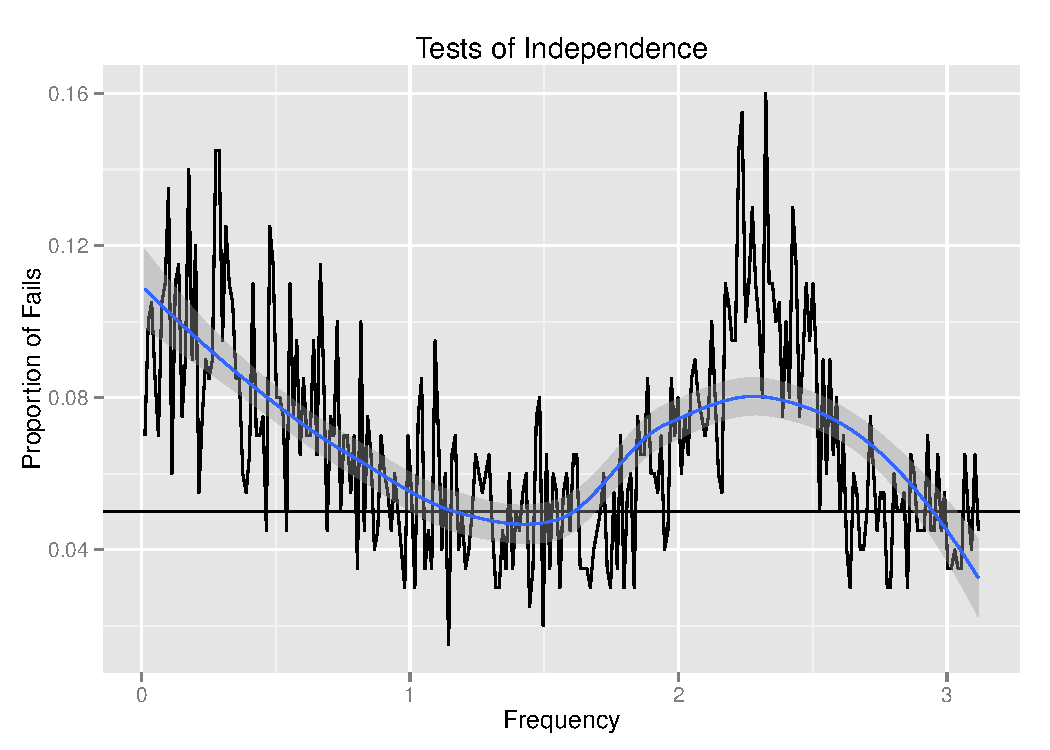
\includegraphics[width=.49\textwidth]{figure/tests-arma421} 
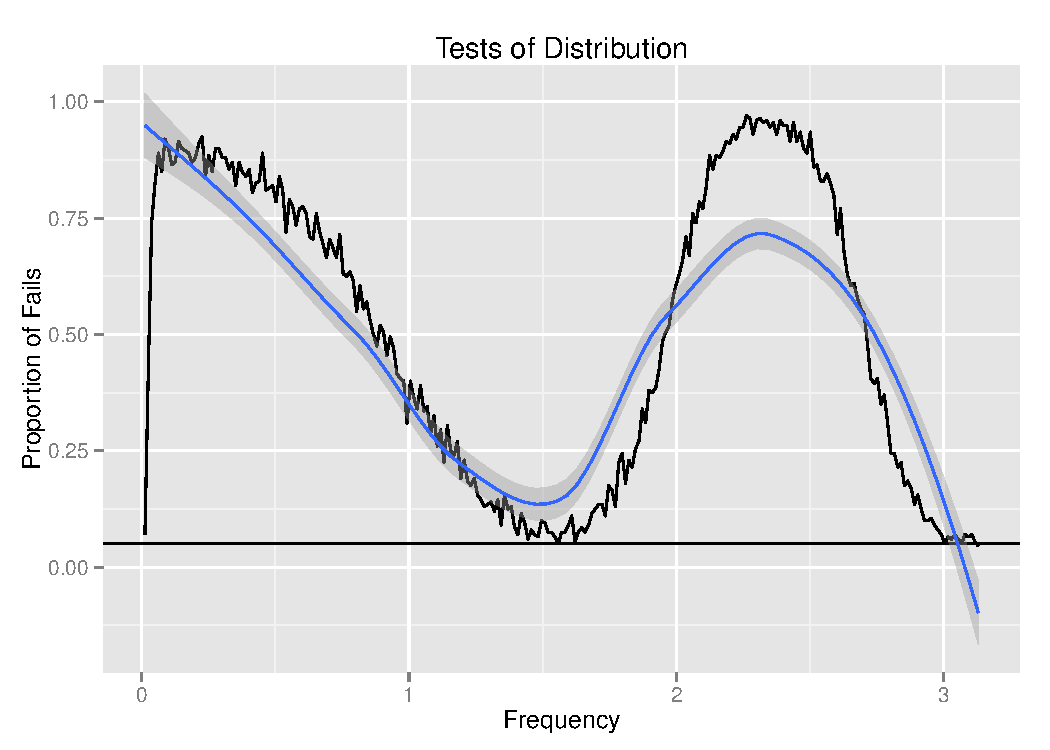
\includegraphics[width=.49\textwidth]{figure/tests-arma422} \caption[Tests of independence and distribution for an ARMA(4,2) model]{Tests of independence and distribution for an ARMA(4,2) model.\label{fig:tests-arma42}}
\end{figure}


\end{knitrout}



\section{Discussion}


\mj{
\paragraph{Issues}
\begin{enumerate}
  \item Multiple comparison 
  \item ARMA(4,2), MA(1), MA(2)
  \item Exponential Fails
  \item Usability 
  \begin{itemize}
    \item ARMA useless, Models w/more structure 
    \item spacing depends on model
    \item can never really be used in practice
  \end{itemize}
  \item Computation time
  \item Pairwise independence $\neq$ Joint independence
\end{enumerate}}


\printbibliography

\end{document}
